\subsection{Implementation}

Zur Umsetzung des WebApp-Wrappers wurden die beiden Frameworks Capacitor und Electron verwendet.
Diese beiden Frameworks bieten eine Reihe von Vorteilen, darunter eine einfache Handhabung, eine weite Verbreitung, einfache Erweiterungsmöglichkeiten, die Möglichkeit, Anwendungen mit \ac{html}, \ac{css} und JavaScript zu erstellen und Schlussendlich die Möglichkeit die Anwendung für alle gängigen Desktop- und Mobile"=Plattformen zu kompilieren.
\cite{capacitor:docs, electron:docs}

Um das Einbinden eines Node.js Projekts zu ermöglichen, wurde das zuvor entwickelte Plugin \hyperref[sec:Capacitor-NodeJS]{Capacitor-NodeJS} verwendet.
Dieses Plugin ermöglicht die Integration eines Node.js Projekts in eine Capacitor Anwendung.
Dadurch können weitere Funktionen mit JavaScript in die Anwendung integriert werden, ohne dass Kenntnisse anderer Programmiersprachen nötig sind.

Um das Einblenden und Steuern von externen Webinhalten zu ermöglichen, wurde das zuvor entwickelte Plugin \hyperref[sec:Capacitor-BrowserView]{Capacitor-BrowserView} verwendet.
Dadurch kann eine externe Webseite in den WebApp-Wrapper integriert werden.

\begin{figure}[H]
  \centering
  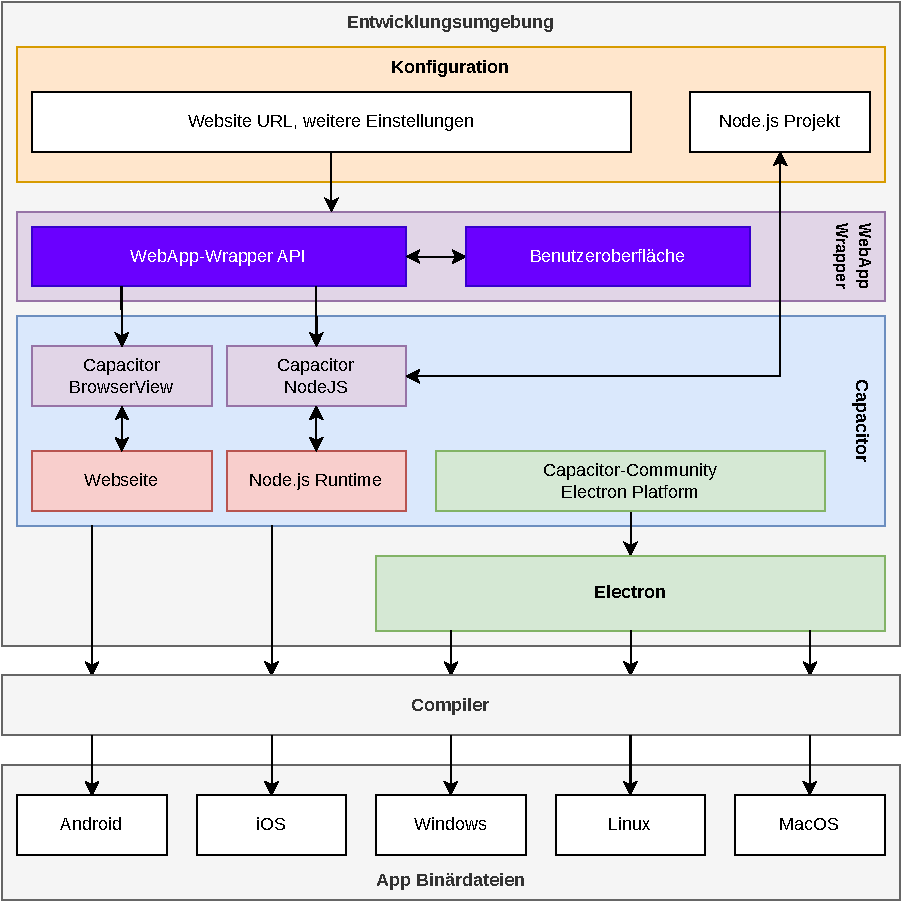
\includegraphics[width=0.9\textwidth]{assets/04_WebApp-Wrapper/01_Implementation.drawio.pdf}
  \caption[WebApp-Wrapper / Implementation]{Implementation des WebApp-Wrappers}
  \label{asset:WebApp-Wrapper:Implementation}
\end{figure}

\newpage

\subsubsection{Konfiguration}

Die Konfiguration ist ein wichtiger Schritt bei der Verwendung des WebApp-Wrappers.
Sie ermöglicht es dem Entwickler, die Anwendung an seine Bedürfnisse anzupassen.

Die wichtigste Konfiguration des WebApp-Wrappers ist die \code{appUrl}.
Dadurch wird festgelegt, welche Webseite in die Anwendung verpackt bzw.\ angezeigt werden soll.
Aus Sicherheitsgründen wird die Navigation ausschließlich auf die Angegebene Webseite beschränkt, externe Webseiten werden in einem externen Browser geöffnet.

Alle verfügbaren Konfigurationen werden im Kapitel \nameref{sec:WebApp-Wrapper:Benutzung} aufgeführt.

\subsubsection{Benutzeroberfläche}

Die Benutzeroberfläche des WebApp-Wrappers wurde mithilfe des PicoCSS Frameworks gestaltet und besteht aus einer optionalen Menüleiste, einem Ladebildschirm, einem Ladebalken, einem Fehlerbildschirm und einem Meldungsfenster:

Der Ladebildschirm wird zu Beginn angezeigt, bis die Webseite vollständig geladen ist oder ein Fehler auftritt.
Wenn die Webseite erfolgreich geladen wurde, wird der Ladebildschirm ausgeblendet und ein Fenster mit der geladenen Webseite (auch BrowserView genannt) wird über die Benutzeroberfläche gelegt, damit der Endbenutzer mit der Webseite interagieren kann.
Bei einem Fehler wird der Ladebildschirm je nach Art des Fehlers durch den entsprechenden Fehlerbildschirm ausgewechselt.
Bei einer fehlenden Internetverbindung wird ein Benutzer-Offline Bildschirm angezeigt.
Bei einem Fehler am Server wird ein Webseite-Offline Bildschirm angezeigt.

Wenn die Webseite erfolgreich geladen wurde und der Endbenutzer auf der Webseite weiter navigiert, wird ein Ladebalken angezeigt, um den Benutzer über den weiteren Ladevorgang zu informieren.
Dazu wird ein Ladebalken auf der Benutzeroberfläche eingeblednet, und die BrowserView wird etwas verkleinert, sonst würde der Ladebalken verdeckt werden.
Nach einem erfolgreichen Laden wird der Ladebalken ausgeblendet und die BrowserView mit der geladnen Webseite wird wieder vergrößert.

Wenn bei einem weiteren Ladevorgang ein Fehler auftritt, wird die BrowserView vollständig ausgeblendet und der entsprechender Fehlerbildschirm wird angezeigt.

Wenn eine Menüleiste konfiguriert wurde, wird sie ganz oben angezeigt.
Bei der Berechnung der Größe der BrowserView, muss die Menüleiste mit berücksichtigt werden, da sie sonst von der BrowserView überdeckt werden könnte.

\newpage

Wenn ein Meldungsfenster über die WebApp-Wrapper \ac{api} eingeblednet wird, wird die BrowserView ausgeblendet um das Meldungsfenster nicht zu überdecken.
Nach dem schließen des Meldungsfensters wird die BrowserView wieder angezeigt, damit der Endbenutzer weiter mit der Webseite agieren kann.
Entwickler können das Meldungsfenster mit den bereits gewohnten Sprachen \ac{html} und \ac{css} über die WebApp-Wrapper \ac{api} anpassen.

\begin{figure}[H]
  \centering
  \includegraphics[width=\textwidth]{assets/04_WebApp-Wrapper/02_Benutzeroberfläche.drawio.pdf}
  \caption[WebApp-Wrapper / Benutzeroberfläche]{Einfache Illustration der Benutzeroberfläche des WebApp-Wrappers}
\end{figure}

Da das Capacitor-BrowserView Plugin das Ausblenden einer BrowserView noch nicht unterstützt, wird als Workaround die Höhe und Breite der BrowserView auf 0\,Pixel gesetzt.
Dies ist vergleichbar mit einem vollständigen Ausblenden.

Wenn der Endbenutzer die Größe des Anwendungsfensters ändert, muss die Größe der BrowserView angepasst werden.
Dazu wird die Größe der BrowserView bei jeder Änderung der Größe des Anwendungsfensters neu berechnet.

Während der Implementierung wurde festgestellt, dass es zu Problemen kommt, wenn die BrowserView die Benutzeroberfläche vollständig überdeckt.
Dadurch können Größenänderungen des Anwendungsfensters nicht mehr erfasst und die Größe der BrowserView nicht neu berechnet werden.
Um dieses Problem zu umgehen, wird um der BrowserView herum allen Seiten ein Pixel freigelassen, damit die Benutzeroberfläche nicht vollständig überdeckt wird.

\newpage

\subsubsection{WebApp-Wrapper API}

Der WebApp-Wrapper stellt eine \ac{api} bereit, um die Kommunikation zwischen der Webseite und dem integrierten Node.js Projekt zu ermöglichen.

Die \ac{api} stellt einen Tunnel zwischen der \ac{api} des Capacitor-BrowserView Plugins und der \ac{api} des Capacitor-NodeJS Plugins dar.
Wenn eine Nachricht von der Webseite über die Capacitor-BrowserView \ac{api} gesendet wird, empfängt der WebApp-Wrapper diese Nachricht und leitet sie, über die Capacitor-NodeJS \ac{api}, an das Node.js Projekt weiter.
Das gleiche Prinzip gilt auch in die andere Richtung.

Darüber hinaus stellt der WebApp-Wrapper eine \ac{api} bereit, um Konfiguration dynamisch zu ändern und ein Meldungsfenster ein- und auszublenden.
Dieser Teil der \ac{api} ist sowohl im Node.js Projekt als auch auf der geladenen Webseite verfügbar.

Um auch im Meldungsfenster bestimmte Aktionen integrieren zu können, wird vom WebApp Wrapper eine simple \ac{api} bereitgestellt um das Meldungsfenster zu schließen oder Nachrichten zur Webseite oder zum Node.js Projekt zu senden.
Diese \ac{api} Methoden können einer Schaltfläche im Meldungsfenster hinterlegt werden.
Somit kann beispielsweise eine Schaltfläche im Meldungsfenster angezeigt werden, um das Meldungsfenster wieder zu schließen, oder um eine Nachricht zum Node.js Projekt zu senden, welche weitere Aktionen ausführt.

Um dem Entwickler zusätzliche Kontrolle über die geladene Webseite zu geben, stellt der WebApp-Wrapper im Node.js Projekt eine \ac{api} bereit, um die Webseite bzw.\ die BrowserView zu steuern.
Dazu werden \ac{api} Methoden des Capacitor-BrowserView Plugins an das Node.js Projekt weitergeleitet.
